\ytset{https://www.youtube.com/watch?v=XXoQBpW7dSs&list=PLtTPtV8SRcxjedflXwNPSI_fxvxwUCjsd}

\section{Spin States in Quantum Dots}

This lecture follows the review article by \cite{Hanson2007}.

\begin{itemize}
    \item Single Quantum Dots:
          \begin{itemize}
              \item Zeeman splitting of spin states in magnetic field.
              \item Spin Filtering
              \item Kondo Effect
          \end{itemize}
    \item Double Quantum Dots:
          \begin{itemize}
              \item Singlet and Triplet States
              \item Pauli Spin Blockade
              \item Spin-orbit and Hyperfine interactions
          \end{itemize}


    \item $N = 1$ excitation spectrum using CSD, you can see jump from grond state to excited state.
    \item You can also see even more states when you apply a magnetic field, which gives Zeeman splitting of spin states \parencite{Hanson2003}.
    \item Let's look at spin states in this figure \ref{fig:spin-states-quantum-dot}.
          \begin{figure}
              \centering
              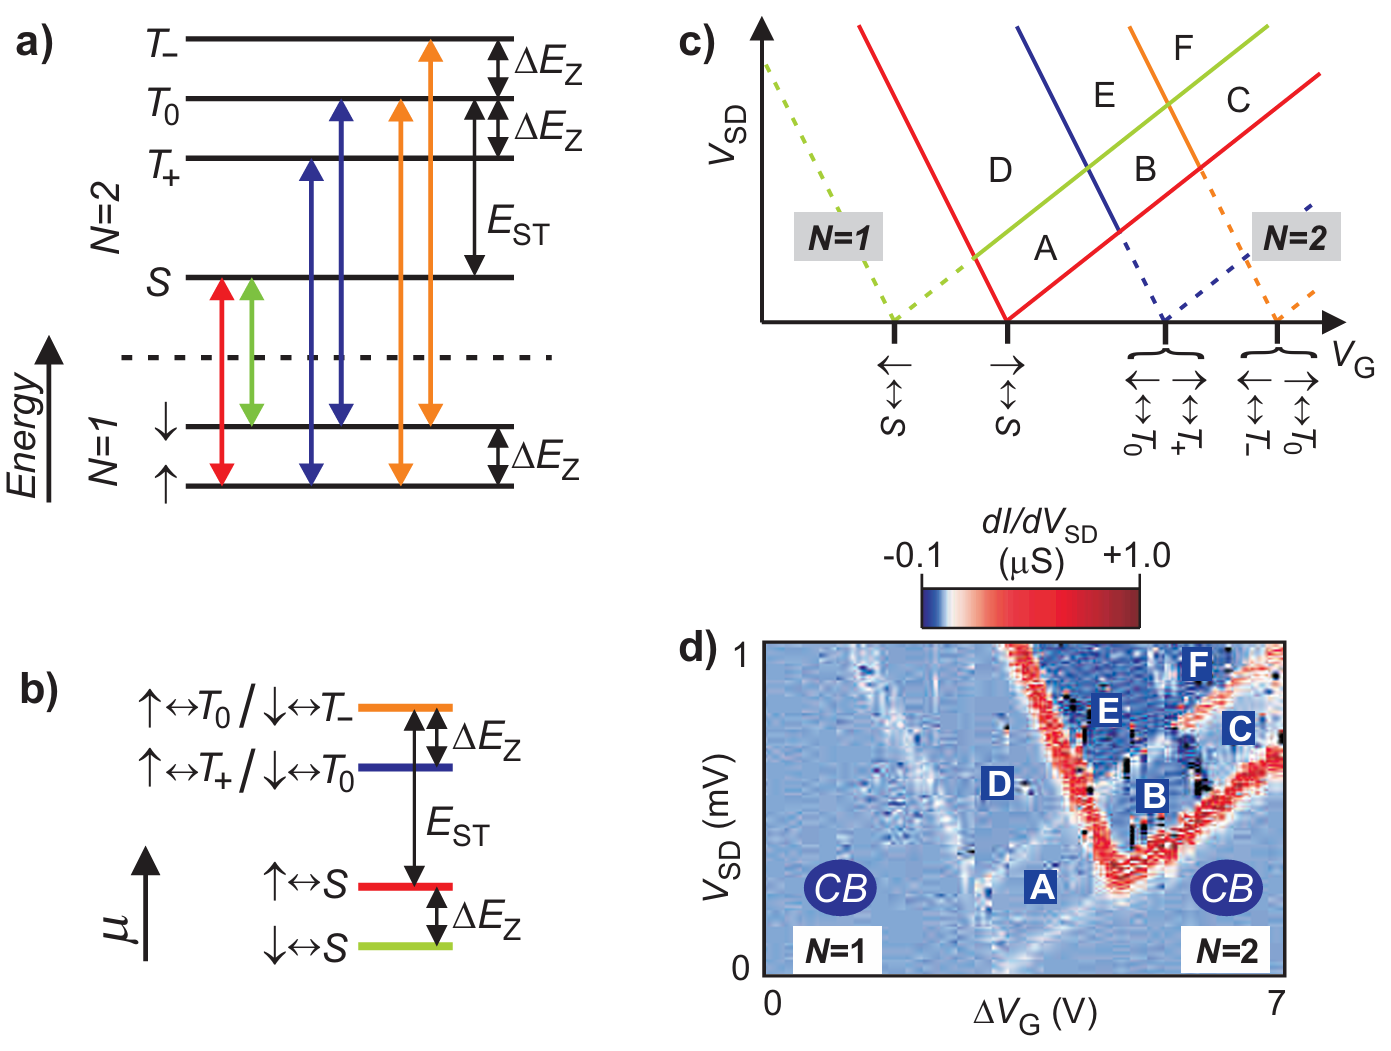
\includegraphics[width=0.6\textwidth]{../Images/spinstatessingledot-1and2electrons-hanson2007.png}
              \caption{Spin states for one and two electrons in a quantum dot \parencite{Hanson2007}.}
              \label{fig:spin-states-quantum-dot}
          \end{figure}
    \item Can make a spin filter which only allows one spin orientation to pass through. Theory \parencite{Recher2000} and experiment \parencite{Folk2003}
    \item Kondo Effect: spin in a quantum dot is `screened' by spins of electrons in the leads. Electrons in the leads form a `Kondo Cloud' of opposite spin.
    \item This is destroyed by finite bias, magnetic field and temperature.
    \item This manifests in QDs as odd fillings having a conductance peak at zero bias via a co-tunneling process \parencite{GoldhaberGordon1998, Cronenwett1998}.
    \item Example of Kondo effect using InAs nanowire quantum dot \parencite{Kretinin2011}
    \item If you apply a magnetic field, you can see the Zeeman splitting of the Kondo peak away from zero bias \parencite{Cronenwett1998}.
    \item Now we move to double quantum dots (DQD).
    \item QPC detector for double dot. The QPC is a tunneling junction between the two dots. QPC detects all charge transitions, also between dots.
    \item Charge stability diagram of DQD. Labels (N\textsubscript{L}, N\textsubscript{R}) refer to number of electrons in left and right dot respectively.
    \item Bias through QPC instead of through the dots.

          \begin{figure}
              \centering
              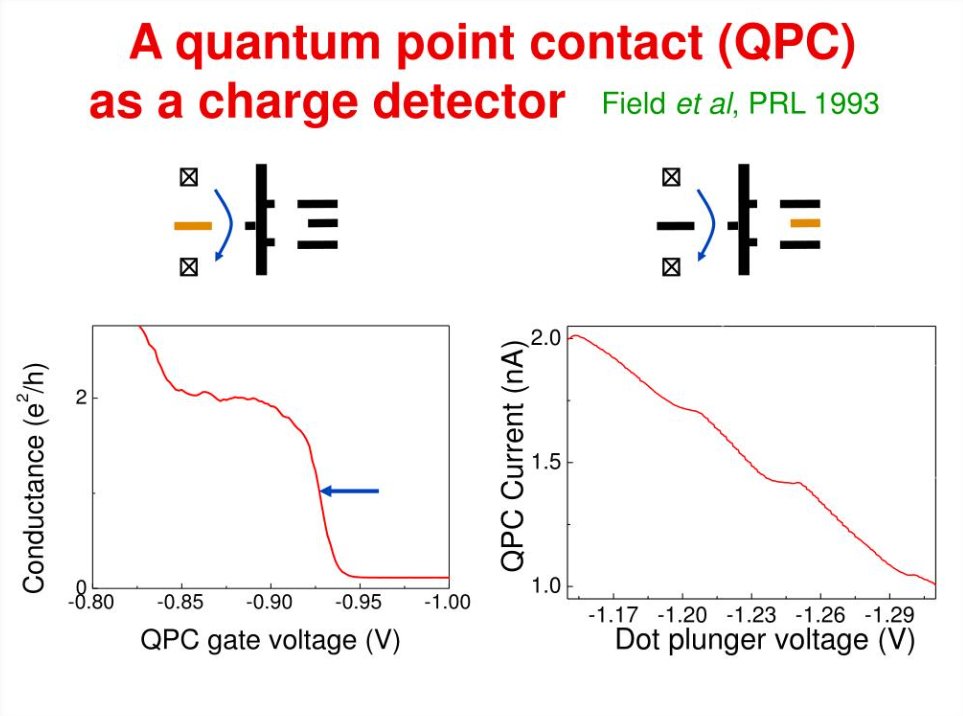
\includegraphics[width=0.6\textwidth]{../Images/QPCs-example.png}
              \caption{QPC as a charge sensor for a quantum dot}
              \label{fig:qpc-example}
          \end{figure}

    \item The group of Lieven Vandersypen at Delft University of Technology has developed an automated algorithm to find the single electron regime using charge sensors (QPCs) (\ylink{37:12}).
    \item Tune gate coltage on QPC until youre at final sensitive drop in conductance \parencite{Field1993}, see example in figure \ref{fig:qpc-example}.
    \item When you add electron to dot, the conductance of the QPC shifts, so that we see a plateau. We can always see the last electron added or removed from the dot using the QPC.
    \item Comparitively the conductance peaks become very small when you reach the last electron in the dot and are hard to see.
    \item Pauli Spin Blockade \parencite{Ono2002}:
          \begin{itemize}
              \item Consider two electrons in a double quantum dot.
              \item If the electrons are in a triplet state, they cannot both occupy the same dot due to Pauli exclusion principle.
              \item This results in a blockade of current through the double dot when trying to move from (1,1) to (0,2) charge configuration.
              \item This effect can be used to read out spin states in quantum dots.
              \item Triplet states: $S = 1$, example: $T_+ = \uparrow\ \uparrow$, $T_- = \downarrow\ \downarrow$, $T_0 = \frac{1}{\sqrt{2}}(\uparrow\ \downarrow + \downarrow\ \uparrow)$
              \item singlet states: $S = 0$, example: $S = \frac{1}{\sqrt{2}}(\uparrow\ \downarrow - \downarrow\ \uparrow)$
          \end{itemize}
    \item By biasing a quantum dot, electrons can flow until the current stops due to the spin blockade. This indicates that a spin triplet state has been formed, which can be used to set the initial state of a qubit (\ylink{50:57}).
    \item Charge stability diagram showing Pauli spin blockade \parencite{NadjPerge2010}.
    \item Microwave photon spectroscopy in quantum dots to see the transitions \parencite{Schreiber2011}
    \item Electron spins in semiconductors:
          \begin{itemize}
              \item Spin-Orbit interaction
              \item Hyperfine interaction
              \item Spin-orbit + phonons = spin relaxation
              \item Dephasing (10-100ns timescale)
          \end{itemize}
    \item Probe spin mixing in the spin blockade regime.
          \begin{itemize}
              \item Fyperfine-induced spin mizing: mixes singlets and triplets near B=0. (nuclear spins have no energy at B=0 no energy different between S and T).
              \item Spin-orbit induced spin mixing: increases with B field (large energy difference = faster relaxation). Note that spin-orbit has no effect at B=0 since time-reversal symmetry is preserved.
          \end{itemize}
    \item Nuclear spin bath dephases electron spin states via hyperfine interaction.
          \begin{equation}
              \mathcal{H} = g \mu_B \vec{B} \vec{S} + \vec{S} \sum_i A_i \vec{I}_i
          \end{equation}
          where A\textsubscript{i} is the hyperfine coupling constant for nucleus i, and I\textsubscript{i} is the nuclear spin operator.
    \item See \parencite{Khaetskii2002, Merkulov2002}
\end{itemize}

